%!TEX program = xelatex

\documentclass[a4paper, openany, oneside]{memoir}
\usepackage[no-math]{fontspec}
\usepackage{pgfplots}
\pgfplotsset{compat=newest}
\usepackage{commath}
\usepackage{mathtools}
\usepackage{amssymb}
\usepackage{amsthm}
\usepackage{booktabs}
\usepackage{mathtools}
\usepackage{xcolor}
\usepackage[separate-uncertainty=true, per-mode=symbol]{siunitx}
\usepackage[noabbrev, capitalize]{cleveref}
\usepackage{listings}
\usepackage[american inductor, european resistor]{circuitikz}
\usepackage{amsmath}
\usepackage{amsfonts}
\usepackage{ifxetex}
\usepackage[dutch,english]{babel}
\usepackage[backend=bibtexu,texencoding=utf8,bibencoding=utf8,style=ieee,sortlocale=en_GB,language=auto]{biblatex}
\usepackage[strict,autostyle]{csquotes}
\usepackage{parskip}
\usepackage{import}
\usepackage{standalone}
\usepackage{hyperref}
%\usepackage[toc,title,titletoc]{appendix}

\ifxetex{} % Fonts laden in het geval dat je met Xetex compiled
    \usepackage{fontspec}
    \defaultfontfeatures{Ligatures=TeX} % To support LaTeX quoting style
    \setromanfont{Palatino Linotype} % Tover ergens in Font mapje in root.
    \setmonofont{Source Code Pro}
\else % Terug val in standaard pdflatex tool chain. Geen ondersteuning voor OTT fonts
    \usepackage[T1]{fontenc}
    \usepackage[utf8]{inputenc}
\fi
\newcommand{\references}[1]{\begin{flushright}{#1}\end{flushright}}
\renewcommand{\vec}[1]{\boldsymbol{\mathbf{#1}}}
\newcommand{\uvec}[1]{\boldsymbol{\hat{\vec{#1}}}}
\newcommand{\mat}[1]{\boldsymbol{\mathbf{#1}}}
\newcommand{\fasor}[1]{\boldsymbol{\tilde{\vec{#1}}}}
\newcommand{\cmplx}[0]{\mathrm{j}}
\renewcommand{\Re}[0]{\operatorname{Re}}
\newcommand{\Cov}{\operatorname{Cov}}
\newcommand{\Var}{\operatorname{Var}}
\newcommand{\proj}{\operatorname{proj}}
\newcommand{\Perp}{\operatorname{perp}}
\newcommand{\col}{\operatorname{col}}
\newcommand{\rect}{\operatorname{rect}}
\newcommand{\sinc}{\operatorname{sinc}}
\newcommand{\IT}{\operatorname{IT}}
\newcommand{\F}{\mathcal{F}}

\newtheorem{definition}{Definition}
\newtheorem{theorem}{Theorem}


\DeclareSIUnit{\voltampere}{VA} %apparent power
\DeclareSIUnit{\pii}{\ensuremath{\pi}}

\hypersetup{%setup hyperlinks
    colorlinks,
    citecolor=black,
    filecolor=black,
    linkcolor=black,
    urlcolor=black
}

% Example boxes
\usepackage{fancybox}
\usepackage{framed}
\usepackage{adjustbox}
\newenvironment{simpages}%
{\AtBeginEnvironment{itemize}{\parskip=0pt\parsep=0pt\partopsep=0pt}
\def\FrameCommand{\fboxsep=.5\FrameSep\shadowbox}\MakeFramed{\FrameRestore}}%
{\endMakeFramed}

% Impulse train
\DeclareFontFamily{U}{wncy}{}
\DeclareFontShape{U}{wncy}{m}{n}{<->wncyr10}{}
\DeclareSymbolFont{mcy}{U}{wncy}{m}{n}
\DeclareMathSymbol{\Sha}{\mathord}{mcy}{"58}
\addbibresource{../../../../includes/bibliography.bib}

\begin{document}

\section{Concept}
The reconstruction poses two specifications for the sampling methods:
\begin{enumerate}
\item all lags in $\mathbb{Z}$ must be available
\item the sampling method must be described by sampling matrix $\mathbf{C}$
\end{enumerate}
We will propose three methods to handle these specifications:
\begin{itemize}
\item \textit{circular sparse ruler}
\item \textit{collaborative sampling}
\item \textit{coprime sampling}
\end{itemize}
each of these techniques impose their own restrictions to the sampling. Circular sparse ruler enforces that the sampling is done by a single device with multiple samplers with the same sample frequency. Collaborative sampling is done with multiple device with multiple samplers with the same sample frequency. Coprime sampling enforces the use of one device with exactly two samplers, but allows for different sampling frequencies. 


% \begin{figure}[H]
%     \centering
%     \begin{tikzpicture}
%         \def\N{7}
%         \draw [thick, black] circle[radius=2.5cm] (0,0);
%         \foreach \i in {1,...,\N} {
%             \draw [scale=1,domain=2.3:2.7,smooth,variable=\x,black,thick] plot ({\x*sin(360*(\i-1)/\N)},{\x*cos(360*(\i-1)/\N)});
%             \draw [black,thick,dashed] (0,0) -- ({2.5*sin(360*(\i-1)/\N)},{2.5*cos(360*(\i-1)/\N)});
%             \node[black] at ({3*sin(360*(\i-1)/\N)},{3*cos(360*(\i-1)/\N)}) {$\i$};
%         }
%         \foreach \i in {0,1,3} {
%             \draw [scale=1,domain=2.3:2.7,smooth,variable=\x,red,line width=1mm] plot ({\x*sin(360*\i/\N)},{\x*cos(360*\i/\N)});
%         }
%         \draw [scale=1,domain=0.1:0.9,smooth,variable=\x,black,thick,>=latex,<->,red] plot ({2*sin(360*\x/\N)},{2*cos(360*\x/\N)}); % 1
%         \draw [scale=1,domain=1.1:2.9,smooth,variable=\x,black,thick,>=latex,<->,red] plot ({2*sin(360*\x/\N)},{2*cos(360*\x/\N)}); % 2
%         \draw [scale=1,domain=3.1:6.9,smooth,variable=\x,black,thick,>=latex,<->,red] plot ({2*sin(360*\x/\N)},{2*cos(360*\x/\N)}); % 4
%         \draw [scale=1,domain=0.1:2.9,smooth,variable=\x,black,thick,>=latex,<->,red] plot ({1.5*sin(360*\x/\N)},{1.5*cos(360*\x/\N)}); % 3
%         \draw [scale=1,domain=3.1:7.9,smooth,variable=\x,black,thick,>=latex,<->,red] plot ({1*sin(360*\x/\N)},{1*cos(360*\x/\N)}); % 5
%         \draw [scale=1,domain=1.1:6.9,smooth,variable=\x,black,thick,>=latex,<->,red] plot ({0.5*sin(360*\x/\N)},{0.5*cos(360*\x/\N)}); % 6
%     \end{tikzpicture}
%     \caption{Minimal circular ruler for $N=7$}
%     \label{fig:circular-ruler}
% \end{figure}

\begin{figure}[H]
\centering
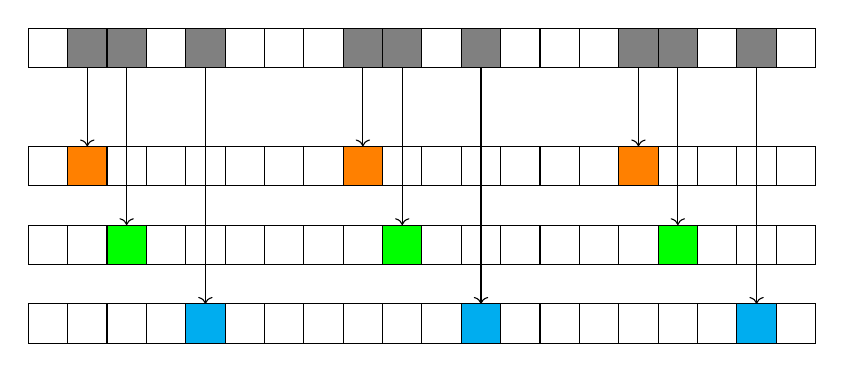
\begin{tikzpicture}
\draw  (-1,0.5) rectangle (-0.5,0);
\draw  [fill=gray](-0.5,0.5) rectangle (0,0);
\draw  [fill=gray](0,0.5) rectangle (0.5,0);
\draw  (0.5,0.5) rectangle (1,0);
\draw  [fill=gray](1,0.5) rectangle (1.5,0);
\draw  (1.5,0.5) rectangle (2,0);
\draw  (2,0.5) rectangle (2.5,0);
\draw  (2.5,0.5) rectangle (3,0);
\draw  [fill=gray](3,0.5) rectangle (3.5,0);
\draw  [fill=gray](3.5,0.5) rectangle (4,0);
\draw  (4,0.5) rectangle (4.5,0);
\draw  [fill=gray](4.5,0.5) rectangle (5,0);
\draw  (5,0.5) rectangle (5.5,0);
\draw  (5.5,0.5) rectangle (6,0);
\draw  (6,0.5) rectangle (6.5,0);
\draw  [fill=gray](6.5,0.5) rectangle (7,0);
\draw  [fill=gray](7,0.5) rectangle (7.5,0);
\draw  (7.5,0.5) rectangle (8,0);
\draw  [fill=gray](8,0.5) rectangle (8.5,0);
\draw  (8.5,0.5) rectangle (9,0);

\draw  (-1,-1) rectangle (-0.5,-1.5);
\draw  [fill=orange](-0.5,-1) rectangle (0,-1.5);
\draw  (0,-1) rectangle (0.5,-1.5);
\draw  (0.5,-1) rectangle (1,-1.5);
\draw  (1,-1) rectangle (1.5,-1.5);
\draw  (1.5,-1) rectangle (2,-1.5);
\draw  (2,-1) rectangle (2.5,-1.5);
\draw  (2.5,-1) rectangle (3,-1.5);
\draw  [fill=orange](3,-1) rectangle (3.5,-1.5);
\draw  (3.5,-1) rectangle (4,-1.5);
\draw  (4,-1) rectangle (4.5,-1.5);
\draw  (4.5,-1) rectangle (5,-1.5);
\draw  (5,-1) rectangle (5.5,-1.5);
\draw  (5.5,-1) rectangle (6,-1.5);
\draw  (6,-1) rectangle (6.5,-1.5);
\draw  [fill=orange](6.5,-1) rectangle (7,-1.5);
\draw  (7,-1) rectangle (7.5,-1.5);
\draw  (7.5,-1) rectangle (8,-1.5);
\draw  (8,-1) rectangle (8.5,-1.5);
\draw  (8.5,-1) rectangle (9,-1.5);

\draw  (-1,-2) rectangle (-0.5,-2.5);
\draw  (-0.5,-2) rectangle (0,-2.5);
\draw  [fill=green](0,-2) rectangle (0.5,-2.5);
\draw  (0.5,-2) rectangle (1,-2.5);
\draw  (1,-2) rectangle (1.5,-2.5);
\draw  (1.5,-2) rectangle (2,-2.5);
\draw  (2,-2) rectangle (2.5,-2.5);
\draw  (2.5,-2) rectangle (3,-2.5);
\draw  (3,-2) rectangle (3.5,-2.5);
\draw  [fill=green](3.5,-2) rectangle (4,-2.5);
\draw  (4,-2) rectangle (4.5,-2.5);
\draw  (4.5,-2) rectangle (5,-2.5);
\draw  (5,-2) rectangle (5.5,-2.5);
\draw  (5.5,-2) rectangle (6,-2.5);
\draw  (6,-2) rectangle (6.5,-2.5);
\draw  (6.5,-2) rectangle (7,-2.5);
\draw  [fill=green](7,-2) rectangle (7.5,-2.5);
\draw  (7.5,-2) rectangle (8,-2.5);
\draw  (8,-2) rectangle (8.5,-2.5);
\draw  (8.5,-2) rectangle (9,-2.5);

\draw  (-1,-3) rectangle (-0.5,-3.5);
\draw  (-0.5,-3) rectangle (0,-3.5);
\draw  (0,-3) rectangle (0.5,-3.5);
\draw  (0.5,-3) rectangle (1,-3.5);
\draw  [fill=cyan](1,-3) rectangle (1.5,-3.5);
\draw  (1.5,-3) rectangle (2,-3.5);
\draw  (2,-3) rectangle (2.5,-3.5);
\draw  (2.5,-3) rectangle (3,-3.5);
\draw  (3,-3) rectangle (3.5,-3.5);
\draw  (3.5,-3) rectangle (4,-3.5);
\draw  (4,-3) rectangle (4.5,-3.5);
\draw  [fill=cyan](4.5,-3) rectangle (5,-3.5);
\draw  (5,-3) rectangle (5.5,-3.5);
\draw  (5.5,-3) rectangle (6,-3.5);
\draw  (6,-3) rectangle (6.5,-3.5);
\draw  (6.5,-3) rectangle (7,-3.5);
\draw  (7,-3) rectangle (7.5,-3.5);
\draw  (7.5,-3) rectangle (8,-3.5);
\draw  [fill=cyan](8,-3) rectangle (8.5,-3.5);
\draw  (8.5,-3) rectangle (9,-3.5);

\draw [->] (-.25,0) to (-.25,-1);
\draw [->] (3.25,0) to (3.25,-1);
\draw [->] (6.75,0) to (6.75,-1);

\draw [->] (.25,0) to (.25,-2);
\draw [->] (3.75,0) to (3.75,-2);
\draw [->] (7.25,0) to (7.25,-2);

\draw [->] (1.25,0) to (1.25,-3);
\draw [->] (4.75,0) to (4.75,-3);
\draw [->] (8.25,0) to (8.25,-3);

\end{tikzpicture}
\caption{circular sparse ruler sampling with three samplers}\label{tkz:circsparseruler}
\end{figure}

\begin{figure}[H]
\centering
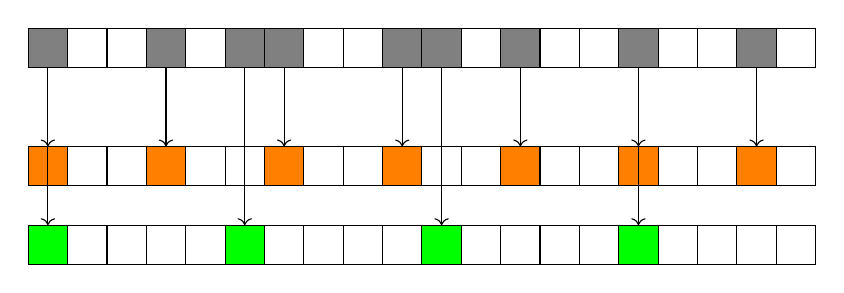
\begin{tikzpicture}
\draw  [fill=gray](-1,0.5) rectangle (-0.5,0);
\draw  (-0.5,0.5) rectangle (0,0);
\draw  (0,0.5) rectangle (0.5,0);
\draw  [fill=gray](0.5,0.5) rectangle (1,0);
\draw  (1,0.5) rectangle (1.5,0);
\draw  [fill=gray](1.5,0.5) rectangle (2,0);
\draw  [fill=gray](2,0.5) rectangle (2.5,0);
\draw  (2.5,0.5) rectangle (3,0);
\draw  (3,0.5) rectangle (3.5,0);
\draw  [fill=gray](3.5,0.5) rectangle (4,0);
\draw [fill=gray] (4,0.5) rectangle (4.5,0);
\draw  (4.5,0.5) rectangle (5,0);
\draw  [fill=gray](5,0.5) rectangle (5.5,0);
\draw  (5.5,0.5) rectangle (6,0);
\draw  (6,0.5) rectangle (6.5,0);
\draw [fill=gray](6.5,0.5) rectangle (7,0);
\draw  (7,0.5) rectangle (7.5,0);
\draw  (7.5,0.5) rectangle (8,0);
\draw  [fill=gray](8,0.5) rectangle (8.5,0);
\draw  (8.5,0.5) rectangle (9,0);

\draw  [fill=orange](-1,-1) rectangle (-0.5,-1.5);
\draw  (-0.5,-1) rectangle (0,-1.5);
\draw  (0,-1) rectangle (0.5,-1.5);
\draw  [fill=orange](0.5,-1) rectangle (1,-1.5);
\draw  (1,-1) rectangle (1.5,-1.5);
\draw  (1.5,-1) rectangle (2,-1.5);
\draw  [fill=orange](2,-1) rectangle (2.5,-1.5);
\draw  (2.5,-1) rectangle (3,-1.5);
\draw  (3,-1) rectangle (3.5,-1.5);
\draw  [fill=orange](3.5,-1) rectangle (4,-1.5);
\draw  (4,-1) rectangle (4.5,-1.5);
\draw  (4.5,-1) rectangle (5,-1.5);
\draw  [fill=orange](5,-1) rectangle (5.5,-1.5);
\draw  (5.5,-1) rectangle (6,-1.5);
\draw  (6,-1) rectangle (6.5,-1.5);
\draw  [fill=orange](6.5,-1) rectangle (7,-1.5);
\draw  (7,-1) rectangle (7.5,-1.5);
\draw  (7.5,-1) rectangle (8,-1.5);
\draw  [fill=orange](8,-1) rectangle (8.5,-1.5);
\draw  (8.5,-1) rectangle (9,-1.5);

\draw  [fill=green](-1,-2) rectangle (-0.5,-2.5);
\draw  (-0.5,-2) rectangle (0,-2.5);
\draw  (0,-2) rectangle (0.5,-2.5);
\draw  (0.5,-2) rectangle (1,-2.5);
\draw  (1,-2) rectangle (1.5,-2.5);
\draw [fill=green] (1.5,-2) rectangle (2,-2.5);
\draw  (2,-2) rectangle (2.5,-2.5);
\draw  (2.5,-2) rectangle (3,-2.5);
\draw  (3,-2) rectangle (3.5,-2.5);
\draw  (3.5,-2) rectangle (4,-2.5);
\draw  [fill=green](4,-2) rectangle (4.5,-2.5);
\draw  (4.5,-2) rectangle (5,-2.5);
\draw  (5,-2) rectangle (5.5,-2.5);
\draw  (5.5,-2) rectangle (6,-2.5);
\draw  (6,-2) rectangle (6.5,-2.5);
\draw [fill=green] (6.5,-2) rectangle (7,-2.5);
\draw  (7,-2) rectangle (7.5,-2.5);
\draw  (7.5,-2) rectangle (8,-2.5);
\draw  (8,-2) rectangle (8.5,-2.5);
\draw  (8.5,-2) rectangle (9,-2.5);

\draw [->] (-.75,0) to (-.75,-1);
\draw [->] (.75,0) to (.75,-1);
\draw [->] (2.25,0) to (2.25,-1);
\draw [->] (3.75,0) to (3.75,-1);
\draw [->] (5.25,0) to (5.25,-1);
\draw [->] (6.75,0) to (6.75,-1);
\draw [->] (8.25,0) to (8.25,-1);

\draw [->] (-.75,0) to (-.75,-2);
\draw [->] (1.75,0) to (1.75,-2);
\draw [->] (4.25,0) to (4.25,-2);
\draw [->] (6.75,0) to (6.75,-2);

\end{tikzpicture}
\caption{coprime sampling with $m=3,n=5$}\label{tkz:coprime}
\end{figure}

\begin{figure}[H]
\centering
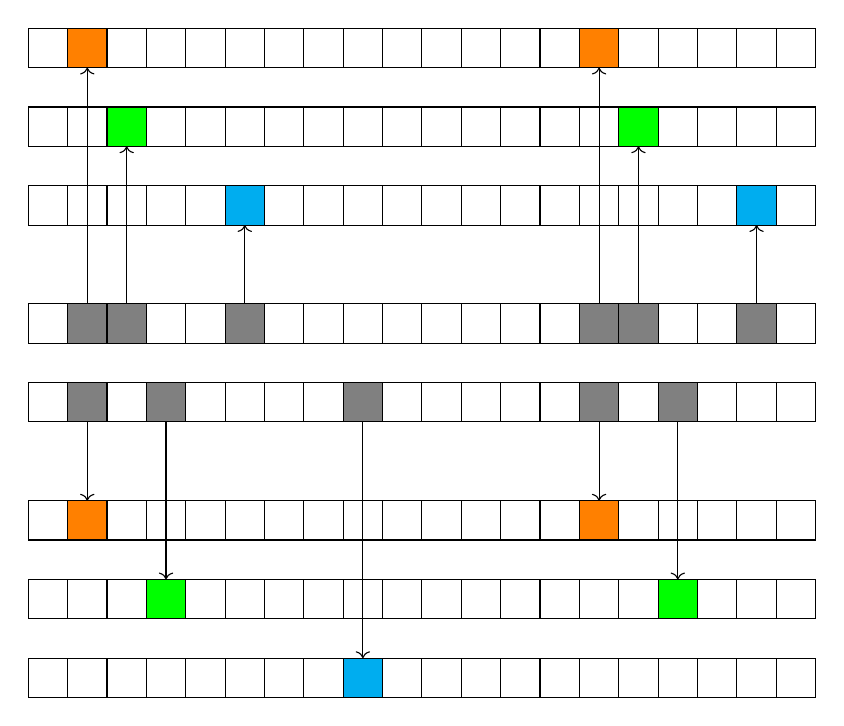
\begin{tikzpicture}
\draw  (-1,-4) rectangle (-0.5,-4.5);
\draw  [fill=gray](-0.5,-4) rectangle (0,-4.5);
\draw  [fill=gray](0,-4) rectangle (0.5,-4.5);
\draw  (0.5,-4) rectangle (1,-4.5);
\draw  (1,-4) rectangle (1.5,-4.5);
\draw  [fill=gray](1.5,-4) rectangle (2,-4.5);
\draw  (2,-4) rectangle (2.5,-4.5);
\draw  (2.5,-4) rectangle (3,-4.5);
\draw  (3,-4) rectangle (3.5,-4.5);
\draw  (3.5,-4) rectangle (4,-4.5);
\draw  (4,-4) rectangle (4.5,-4.5);
\draw  (4.5,-4) rectangle (5,-4.5);
\draw  (5,-4) rectangle (5.5,-4.5);
\draw  (5.5,-4) rectangle (6,-4.5);
\draw  [fill=gray](6,-4) rectangle (6.5,-4.5);
\draw  [fill=gray](6.5,-4) rectangle (7,-4.5);
\draw  (7,-4) rectangle (7.5,-4.5);
\draw  (7.5,-4) rectangle (8,-4.5);
\draw  [fill=gray](8,-4) rectangle (8.5,-4.5);
\draw  (8.5,-4) rectangle (9,-4.5);

\draw  (-1,-0.5) rectangle (-0.5,-1);
\draw  [fill=orange](-0.5,-0.5) rectangle (0,-1);
\draw  (0,-0.5) rectangle (0.5,-1);
\draw  (0.5,-0.5) rectangle (1,-1);
\draw  (1,-0.5) rectangle (1.5,-1);
\draw  (1.5,-0.5) rectangle (2,-1);
\draw  (2,-0.5) rectangle (2.5,-1);
\draw  (2.5,-0.5) rectangle (3,-1);
\draw  (3,-0.5) rectangle (3.5,-1);
\draw  (3.5,-0.5) rectangle (4,-1);
\draw  (4,-0.5) rectangle (4.5,-1);
\draw  (4.5,-0.5) rectangle (5,-1);
\draw  (5,-0.5) rectangle (5.5,-1);
\draw  (5.5,-0.5) rectangle (6,-1);
\draw  [fill=orange](6,-0.5) rectangle (6.5,-1);
\draw  (6.5,-0.5) rectangle (7,-1);
\draw  (7,-0.5) rectangle (7.5,-1);
\draw  (7.5,-0.5) rectangle (8,-1);
\draw  (8,-0.5) rectangle (8.5,-1);
\draw  (8.5,-0.5) rectangle (9,-1);

\draw  (-1,-1.5) rectangle (-0.5,-2);
\draw  (-0.5,-1.5) rectangle (0,-2);
\draw  [fill=green](0,-1.5) rectangle (0.5,-2);
\draw  (0.5,-1.5) rectangle (1,-2);
\draw  (1,-1.5) rectangle (1.5,-2);
\draw  (1.5,-1.5) rectangle (2,-2);
\draw  (2,-1.5) rectangle (2.5,-2);
\draw  (2.5,-1.5) rectangle (3,-2);
\draw  (3,-1.5) rectangle (3.5,-2);
\draw  (3.5,-1.5) rectangle (4,-2);
\draw  (4,-1.5) rectangle (4.5,-2);
\draw  (4.5,-1.5) rectangle (5,-2);
\draw  (5,-1.5) rectangle (5.5,-2);
\draw  (5.5,-1.5) rectangle (6,-2);
\draw  (6,-1.5) rectangle (6.5,-2);
\draw  [fill=green](6.5,-1.5) rectangle (7,-2);
\draw  (7,-1.5) rectangle (7.5,-2);
\draw  (7.5,-1.5) rectangle (8,-2);
\draw  (8,-1.5) rectangle (8.5,-2);
\draw  (8.5,-1.5) rectangle (9,-2);

\draw  (-1,-2.5) rectangle (-0.5,-3);
\draw  (-0.5,-2.5) rectangle (0,-3);
\draw  (0,-2.5) rectangle (0.5,-3);
\draw  (0.5,-2.5) rectangle (1,-3);
\draw  (1,-2.5) rectangle (1.5,-3);
\draw  [fill=cyan](1.5,-2.5) rectangle (2,-3);
\draw  (2,-2.5) rectangle (2.5,-3);
\draw  (2.5,-2.5) rectangle (3,-3);
\draw  (3,-2.5) rectangle (3.5,-3);
\draw  (3.5,-2.5) rectangle (4,-3);
\draw  (4,-2.5) rectangle (4.5,-3);
\draw  (4.5,-2.5) rectangle (5,-3);
\draw  (5,-2.5) rectangle (5.5,-3);
\draw  (5.5,-2.5) rectangle (6,-3);
\draw  (6,-2.5) rectangle (6.5,-3);
\draw  (6.5,-2.5) rectangle (7,-3);
\draw  (7,-2.5) rectangle (7.5,-3);
\draw  (7.5,-2.5) rectangle (8,-3);
\draw  [fill=cyan](8,-2.5) rectangle (8.5,-3);
\draw  (8.5,-2.5) rectangle (9,-3);

\draw [->] (-0.25,-4) to (-0.25,-1);
\draw [->] (6.25,-4) to (6.25,-1);

\draw [->] (0.25,-4) to (0.25,-2);
\draw [->] (6.75,-4) to (6.75,-2);

\draw [->] (1.75,-4) to (1.75,-3);
\draw [->] (8.25,-4) to (8.25,-3);

\draw  (-1,-5) rectangle (-0.5,-5.5);
\draw  [fill=gray](-0.5,-5) rectangle (0,-5.5);
\draw  (0,-5) rectangle (0.5,-5.5);
\draw  [fill=gray](0.5,-5) rectangle (1,-5.5);
\draw  (1,-5) rectangle (1.5,-5.5);
\draw  (1.5,-5) rectangle (2,-5.5);
\draw  (2,-5) rectangle (2.5,-5.5);
\draw  (2.5,-5) rectangle (3,-5.5);
\draw  [fill=gray](3,-5) rectangle (3.5,-5.5);
\draw  (3.5,-5) rectangle (4,-5.5);
\draw  (4,-5) rectangle (4.5,-5.5);
\draw  (4.5,-5) rectangle (5,-5.5);
\draw  (5,-5) rectangle (5.5,-5.5);
\draw  (5.5,-5) rectangle (6,-5.5);
\draw  [fill=gray](6,-5) rectangle (6.5,-5.5);
\draw  (6.5,-5) rectangle (7,-5.5);
\draw  [fill=gray](7,-5) rectangle (7.5,-5.5);
\draw  (7.5,-5) rectangle (8,-5.5);
\draw  (8,-5) rectangle (8.5,-5.5);
\draw  (8.5,-5) rectangle (9,-5.5);

\draw  (-1,-6.5) rectangle (-0.5,-7);
\draw  [fill=orange](-0.5,-6.5) rectangle (0,-7);
\draw  (0,-6.5) rectangle (0.5,-7);
\draw  (0.5,-6.5) rectangle (1,-7);
\draw  (1,-6.5) rectangle (1.5,-7);
\draw  (1.5,-6.5) rectangle (2,-7);
\draw  (2,-6.5) rectangle (2.5,-7);
\draw  (2.5,-6.5) rectangle (3,-7);
\draw  (3,-6.5) rectangle (3.5,-7);
\draw  (3.5,-6.5) rectangle (4,-7);
\draw  (4,-6.5) rectangle (4.5,-7);
\draw  (4.5,-6.5) rectangle (5,-7);
\draw  (5,-6.5) rectangle (5.5,-7);
\draw  (5.5,-6.5) rectangle (6,-7);
\draw  [fill=orange](6,-6.5) rectangle (6.5,-7);
\draw  (6.5,-6.5) rectangle (7,-7);
\draw  (7,-6.5) rectangle (7.5,-7);
\draw  (7.5,-6.5) rectangle (8,-7);
\draw  (8,-6.5) rectangle (8.5,-7);
\draw  (8.5,-6.5) rectangle (9,-7);

\draw  (-1,-7.5) rectangle (-0.5,-8);
\draw  (-0.5,-7.5) rectangle (0,-8);
\draw  (0,-7.5) rectangle (0.5,-8);
\draw  [fill=green](0.5,-7.5) rectangle (1,-8);
\draw  (1,-7.5) rectangle (1.5,-8);
\draw  (1.5,-7.5) rectangle (2,-8);
\draw  (2,-7.5) rectangle (2.5,-8);
\draw  (2.5,-7.5) rectangle (3,-8);
\draw  (3,-7.5) rectangle (3.5,-8);
\draw  (3.5,-7.5) rectangle (4,-8);
\draw  (4,-7.5) rectangle (4.5,-8);
\draw  (4.5,-7.5) rectangle (5,-8);
\draw  (5,-7.5) rectangle (5.5,-8);
\draw  (5.5,-7.5) rectangle (6,-8);
\draw  (6,-7.5) rectangle (6.5,-8);
\draw  (6.5,-7.5) rectangle (7,-8);
\draw  [fill=green](7,-7.5) rectangle (7.5,-8);
\draw  (7.5,-7.5) rectangle (8,-8);
\draw  (8,-7.5) rectangle (8.5,-8);
\draw  (8.5,-7.5) rectangle (9,-8);

\draw  (-1,-8.5) rectangle (-0.5,-9);
\draw  (-0.5,-8.5) rectangle (0,-9);
\draw  (0,-8.5) rectangle (0.5,-9);
\draw  (0.5,-8.5) rectangle (1,-9);
\draw  (1,-8.5) rectangle (1.5,-9);
\draw  (1.5,-8.5) rectangle (2,-9);
\draw  (2,-8.5) rectangle (2.5,-9);
\draw  (2.5,-8.5) rectangle (3,-9);
\draw  [fill=cyan](3,-8.5) rectangle (3.5,-9);
\draw  (3.5,-8.5) rectangle (4,-9);
\draw  (4,-8.5) rectangle (4.5,-9);
\draw  (4.5,-8.5) rectangle (5,-9);
\draw  (5,-8.5) rectangle (5.5,-9);
\draw  (5.5,-8.5) rectangle (6,-9);
\draw  (6,-8.5) rectangle (6.5,-9);
\draw  (6.5,-8.5) rectangle (7,-9);
\draw  (7,-8.5) rectangle (7.5,-9);
\draw  (7.5,-8.5) rectangle (8,-9);
\draw  (8,-8.5) rectangle (8.5,-9);
\draw  (8.5,-8.5) rectangle (9,-9);

\draw [->] (-0.25,-5.5) to (-0.25,-6.5);
\draw [->] (6.25,-5.5) to (6.25,-6.5);

\draw [->] (0.75,-5.5) to (0.75,-7.5);
\draw [->] (7.25,-5.5) to (7.25,-7.5);

\draw [->] (3.25,-5.5) to (3.25,-8.5);

\end{tikzpicture}
\caption{collaborative sampling with two devices with each three samplers}\label{tkz:collaborative}
\end{figure}

\end{document}

